\documentclass[9pt,twocolumn,twoside]{../../styles/osajnl}
\usepackage{fancyvrb}
\journal{i524} 

\title{A Report on Apache Apex}

\author[1]{Srikanth Ramanam}


\affil[1]{School of Informatics and Computing, Bloomington, IN 47408, U.S.A.}


\affil[*]{Corresponding authors: srikrama@iu.edu}

\dates{ \today}

\ociscodes{Stream, Processing, YARN, Apache, Apex, Malhar, I524}



% replace this with your url in github/gitlab
\doi{\url{https://github.com/cloudmesh/sp17-i524/raw/master/paper2/S17-IR-2028/report-review.pdf}}

\begin{abstract}
Apache Apex is a Hadoop YARN native big data processing platform with both stream and batch processing capabilities. This paper explores the architecture, functioning and competition of Apache Apex.
\newline
\end{abstract}

\setboolean{displaycopyright}{true}

\begin{document}

\maketitle

\section{Introduction}
Apache Apex was developed to address the enterprises need to process and analyze real time data stream. It was initially developed by DataTorrent as the core engine for their RTS platform, a platform for processing, analysis and visualization of stream data. DataTorrent later decided to make it open source and submitted the proposal for Apache Apex to Apache incubator in 2015 \cite{www-datatorrentapex}. Apache Apex was accepted to the Apache Incubator and later several enterprises CapitalOne, DirecTV, General Electric, Apple and Silver Spring Networks joined its open source community. Apache Apex was first released in 2016. Apache Apex is built over YARN and is compatible with existing Hadoop platforms.







\section{Components}
Apex has two main components \cite{www-apacheapexwiki}.
\subsection{Apex Core}
Apex Core is the framework for building distributed applications on Hadoop.
\subsection{Apex Malhar}
Malhar provides a library of operators. They are mainly of two types
\subsubsection{Input/Output Operators}
Input/Output operators: These operators offer connectivity with a variety of existing data sources.
\subsubsection{Compute Operators}
Compute Operators: These operators offer functionality of Machine Learning, Stats and Math, Pattern Marching, Query and Scripting, Stream manipulators, Parsers and UI \& Charting.
\begin{figure}[ht!]
\centering
\fbox{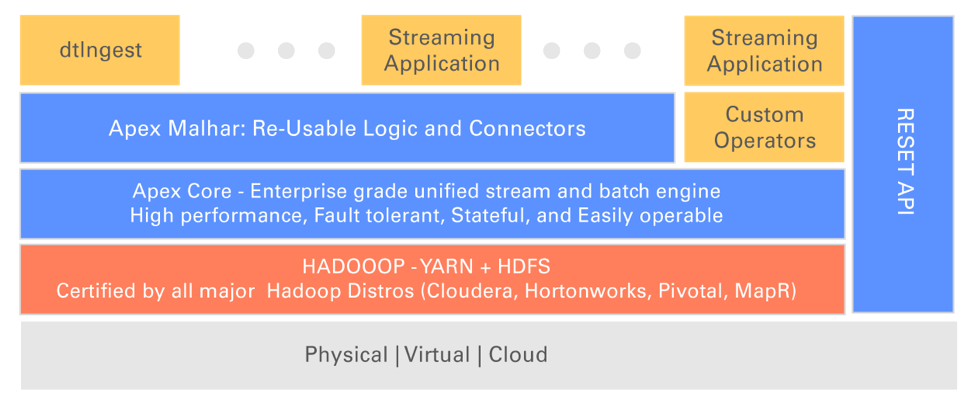
\includegraphics[width=\linewidth]{images/apache-apex-easily-reused.png}}
\caption{Apache Apex Components \cite{www-apacheapexblog}}
\label{fig:Apache Apex Components}
\end{figure}




\section{Architecture}

Operators are the basic blocks of Apex applications. A streaming application is built using in-built or custom operators are connected to form a DAG (Directed Acyclic Graph) using streams. 
\begin{figure}[ht!]
\centering
\fbox{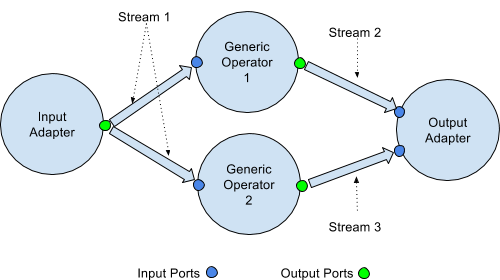
\includegraphics[width=\linewidth]{images/DAG.png}}
\caption{Apex Application DAG \cite{www-apacheapexappdevdoc}}
\label{fig:Apex Application DAG}
\end{figure}



\section{Application Development}
Apex applications can be written in Java using any IDE supporting Java like Eclipse.
Other prerequisites include Apache Maven 3.0., Apache Apex, Apache Malhar \cite{www-apacheapexappdevdoc}.

\subsubsection{Operators}
Operators are independent units of logical operations that either contribute to a part of or a whole business use case. An operator has an input port to receive data tuples and an output port to send data tuples to another operator  or external system \cite{www-apacheapexoperatordoc}.
Types of Operators \cite{www-apacheapexoperatordoc}:
\begin{itemize}
  \item Input Adapter:  An operator at the beginning of the DAG to receive data from an external system.
  \item  Generic Operator: Accepts tuples from previous operator in DAG and does some processing task and outputs the processed data to another operator.
  \item An operator at the end of a DAG and outputs the data tuples to an external system. 
  
\end{itemize}

API \cite{www-apacheapexoperatordoc}:
\begin{itemize}
  \item setup() initializes the operator.
  \item process()  performs the core processing operations on data tuples and gets triggered when tuples are received.
  \item beginWindow()  and endWindow() are used for pre and post processing steps.
  \item teardown() shuts down the operator and releases the resources held by the operator.
\end{itemize}
\subsubsection{Directed Acyclic Graph}
A DAG is constructed to accomplish a business task using several operators connected through streams \cite{www-apacheapexappdevdoc}.

Constructing a DAG:
\begin{itemize}
  \item Operators are added to a DAG using dag.addOperator(args) \cite{ww-apacheapexinslideshare}.
  \item Streams are added to a DAG using dag.addStream(args) \cite{ww-apacheapexinslideshare}.
  \item Other configurations related to YARN can also be added to DAG \cite{ww-apacheapexinslideshare}. 
  
\end{itemize}
\subsubsection{Package}
Apex applications are assembled and shared using Apache Apex Packages, which are zip files with all necessary files to launch those applications.
Apache Apex Packages are created using Maven.                 
First a Maven project is created with path to the application code. 
Then a mvn package command creates an application package in the target package.


Zip structure of a mvn package:
\begin{itemize}
  \item app contains jar files of the DAG code
  \item lib contains jar files of dependencies
  \item conf contains preset configuration
  \item  META-INF contains meta information in files MANIFEST.MF and properties.xml
   \item resources for other files
\end{itemize}


\section{Functioning}
Apex applications are usually packaged, shared and are usually deployed over Hadoop clusters. It is also compatible with several popular data sources as shown in the below figure.
\begin{figure}[ht!]
\centering
\fbox{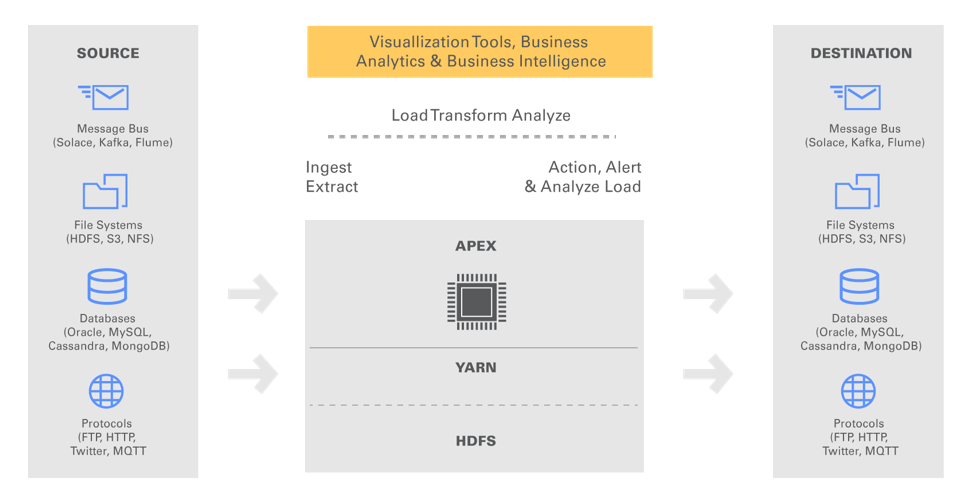
\includegraphics[width=\linewidth]{images/apache-apex-ease-of-integration.png}}
\caption{Apache Apex Interoperability\cite{www-apacheapexblog}}
\label{fig:Apache Apex Interoperability}
\end{figure}

\begin{figure}[ht!]
\centering
\fbox{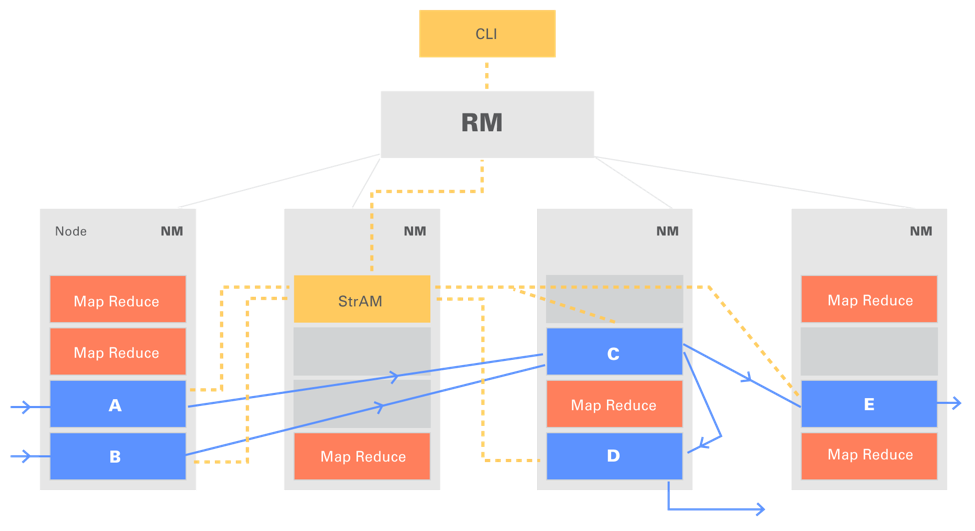
\includegraphics[width=\linewidth]{images/apex-application-in-hadoop-cluster.png}}
\caption{Apache Apex Application Example \cite{www-apacheapexblog}}
\label{fig:Apache Apex Application Example}
\end{figure}
\section{User Interface}
A command line interface called Apex CLI is available for Apache Apex.
It can be launched with command  apex.
help command is available for all commands to obtain information and syntax.
Real-time visualization dashboards can be plugged into applications for visual analytics.


\section{License}
Apache Apex is licensed under Apache License 2.0 \cite{www-apacheapexsite}.  

\section{Pricing}
Apache Apex is a free open source software.
\section{Competition}
Some of the competitors of Apache Apex for stream processing and analytics are \cite{www-apacheapexcompetition}:
\subsection{Apache Spark}
 This is a large-scale data processing engine that also offers stream processing \cite{www-apachesparksite}. But this is not a pure streaming engine as it accomplishes the same through micro-batching, fast execution of batches on small sets of data. 
\subsection{Apache Flink}
This is an open-source stream processing framework that processes streams in real-time \cite{www-apacheapexflink}. Almost similar to Apex but not as widely used.
\subsection{Apache Storm}
This is a free and open source distributed real-time computation system \cite{www-apachestormsite}. This is fast but not stateful like Apex.
\subsection{Apache Samza}
This is a distributed stream processing framework \cite{www-apachesamzasite}. It was first developed by LinkedIn and later opensourced.
\section{Users}
Enterprises like GE, PubMatic, SilverSpring Networks are using Apex based streaming solutions. 
\section{Conclusion}
Apache Apex is an open source YARN(Hadoop 2.0)-native platform \cite{www-apacheapexwiki}. It unifies cloud and batch processing. It can be used for processing both streams of data and static files making it more relevant in the context of present day internet and social media. It is aimed at leveraging the present Hadoop platform and reducing the learning curve for development of applications over it. It is aimed at It can used through a simple API. It enables reuse of code by not having to make drastic changes to the applications by providing interoperability with existing technology stack. It leverages the existing Hadoop platform investments.



\section*{Acknowledgements}

This paper has been written as part of a class assignment for the course: 
I524: Big Data Software and projects, Spring 2017, School of Informatics and computing, Indiana University, Bloomington.
Special thanks to Professor Gregor von Laszewski, Dimitar Nikolov and all associate instructors for guiding through the process of writing this paper.


% Bibliography

\bibliography{references}
 
\end{document}









